% a-project.tex, v-1.0.3 marcoreis baseado no
% abntex2-modelo-trabalho-academico.tex, v-1.9.7 laurocesar
% Copyright 2012-2018 by abnTeX2 group at http://www.abntex.net.br/ 
% 
% This work consists of the files ........
% 
% -----------------------------------------------------------------------------
% Modelo para desenvolvimento de documentação de projetos acadêmicos
% (tese de doutorado, dissertação de mestrado e trabalhos de monografias em geral) 
% em conformidade com ABNT NBR 14724:2011: Informação e documentação. 
% -----------------------------------------------------------------------------
% Opções para a documentação
%
% Fancy page headings 
%\documentclass[fancyheadings, subook]{Classes/a-prj}
%\documentclass[fancyheadings, sureport]{Classes/a-prj}
%
% Fancy chapters and sections headings 
%\documentclass[fancychapter, subook]{Classes/a-prj}
%\documentclass[fancychapter, sureport]{Classes/a-prj}
%
% Fancy page , chapters and sections headings
%\documentclass[fancyheadings, fancychapter, subook]{Classes/a-prj}
\documentclass[fancyheadings, fancychapter, sureport]{Classes/a-prj}
%
% -----------------------------------------------------------------------------
% Alguns comandos para a fancy page headings)
%
% Page header line width
%\footlinewidth{value}
%
% Page footer line width
%\headlinewidth{value}
%
% Page header and footer line width
%\headingslinewidth{value}
%
% Page header and footer lines without text
%\headingslinesonly
%
% The default line width is 0.3pt.
% Set the value to 0pt to remove the page header and/or footer line
%
% -------------------------------------------------------------------------------
% Formato de figuras suportado
% -------------------------------------------------------------------------------
% O formato das figuras depende da forma como o arquivo de saída é gerado.
% As figuras inseridas na pasta Figures serão automaticamente reconhecidas sem
% a necessidade de inserir a extensão do arquivo.
%
% O pdfLaTEX (PDF) suporta figuras com as extensões: pdf, jpg, png e mps.
%
% -------------------------------------------------------------------------------
% Árvore do diretório a-project.tex
%  Diretório
%       \Classes        (requerido)
%       \Figures        (requerido) --------------------------------->
%       \Figures\PDF    (optional)
%       \Figures\JPG    (optional) Figures located within these
%       \Figures\PNG    (optional) folders are searched automatically
%       \Figures\MPS    (optional)  by the a-prj class.
%       \Figures\EPS    (optional)
%       \Figures\PS     (optional) <--------------------------------
%       \Tables         (requerido)
%       \Others         (requerido)
%       \Chapters       (requerido)
%       \Appendices     (optional)
%       \References     (requerido)
%
% -------------------------------------------------------------------------------
% PDF File resumo
\ifpdf
    \hypersetup{
    	backref,
        colorlinks  = true,
        pdftitle    = Modelo de documentação,
        pdfauthor   = {Marco Reis, marco.a.reis@gmail.com},
        pdfsubject  = Mestre em Engenharia,
        pdfcreator  = Subtitulo,
        pdfproducer = PDFLatex,
        pdfkeywords = {documentação, latex, dissertação, tese}}
 \fi
%
% -------------------------------------------------------------------------------
% Relação de pacotes opcionais utilizados
\usepackage[utf8]{inputenc}
\usepackage[brazil]{babel}
\usepackage{longtable}
\usepackage{dcolumn}
\usepackage{multirow}
\usepackage{lscape}
%\usepackage{graphicx}
\usepackage{rotating}
%\usepackage{float,subfigure}
%\usepackage{graphicx, subfigure}
\usepackage{cite}
\usepackage[left=3cm,top=3cm,right=2cm,bottom=2cm]{geometry}
\usepackage[alf]{abntex2cite}
\usepackage{ifpdf}
\usepackage{shadow}
\usepackage{wrapfig}
\usepackage[normalem]{ulem}
\usepackage{makeidx}
\usepackage{yfonts}
\usepackage{algorithm}
\usepackage{algorithmic}
\usepackage{lmodern}
\usepackage[T1]{fontenc}
\usepackage{indentfirst}
\usepackage{color}
\usepackage{microtype}
\usepackage{lipsum}
\usepackage{caption}
\usepackage{subcaption}
\usepackage{pdfpages}

%
\makeindex 
\setlength{\LTcapwidth}{\textwidth}
%
\newtheorem{theorem}{Teorema}
\newtheorem{definition}[theorem]{Definição}
%
% -------------------------------------------------------------------------------
% Configurações do pacote backref
\renewcommand{\backrefpagesname}{Citado na(s) página(s):~}
% Texto padrão antes do número das páginas
\renewcommand{\backref}{}
% Define os textos da citação
\renewcommand*{\backrefalt}[4]{
	\ifcase #1 %
		Nenhuma citação no texto.%
	\or
		Citado na página #2.%
	\else
		Citado #1 vezes nas páginas #2.%
	\fi
}
% 
% -------------------------------------------------------------------------------
% Início do documento raiz
\begin{document}
% Definição do título da página
    \university{Centro Universitário SENAI CIMATEC}
	%\faculty{Programa de...}
	%\school{Escola de...}
% 
    %\course{Engenharia Elétrica}
    %\typework{Relatório Final do Curso de Pós Graduação em Robótica e Sistemas Autônomos}
% 
	\course{Pós-Graduação em Robótica e Sistemas Autônomos}
	%\typework{Disserta\c{c}\~ao de mestrado}
	%\typework{Exame de Qualificação de Mestrado}
% 
	%\course{Engenharia Elétrica}
	%\typework{Tese de doutorado}
	%\typework{Exame de Qualificação de doutorado}
%
% -------------------------------------------------------------------------------
% Informações gerais
    \thesistitle{Relatório Final do Curso}
    \hidevolume
    \thesisvolume{Volume 1 of 1}
    \thesisauthor{Jéssica Lima Motta}
    \thesisauthorr{John Nash}
    \thesisauthorrr{James Clerk Maxwell}
    \thesisauthorrrr{Nikola Tesla}
    \thesisauthorrrrr{Sir Isaac Newton}
    %\thesisadvisor{Prof. Marco Reis, M.Eng.}
    %\hidecoadvisor
    %\thesiscoadvisor{Marco Reis}
    \thesisdegreetitle{Bacharel em Engenharia}
    \thesismonthyear{Dezembro de 2020}
% 
    \maketitlepage
%
% ----------------------------------------------------------------------------
% Inserir Folha de rosto, Nota de estilo, folha de assinaturas, dedicatoria
    \begin{folharosto}

\begin{center}
\theauthor \\
\theauthorr \\
\theauthorrr \\
\theauthorrrr \\
\theauthorrrrr \\
\end{center}
\ \\
\ \\
\ \\
\ \\
\ \\
\begin{spacing}{2}
   \begin{center}
   {\LARGE {\bf \thetitle}}
   \end{center}
\end{spacing}
\ \\
\ \\
\ \\
\vspace*{85mm}
% \begin{flushright}

%    \begin{list}{}{
%       \setlength{\leftmargin}{7.5cm}
%       \setlength{\rightmargin}{0cm}
%       \setlength{\labelwidth}{0pt}
%       \setlength{\labelsep}{\leftmargin}}

%       \item \thetypework apresentada ao \thefaculty, Curso de \thecourse
%       do \theuniversity, como requisito parcial para a obten\c{c}\~ao do
%       t\'itulo de {\bf \thedegreetitle}.

%       \begin{list}{}{
%       \setlength{\leftmargin}{0cm}
%       \setlength{\rightmargin}{0cm}
%       \setlength{\labelwidth}{0pt}
%       \setlength{\labelsep}{\leftmargin}}

%       \item \'Area de conhecimento: Interdisciplinar

%       \item Orientador: \theadvisor
%       \newline \hspace*{2.1cm}  %{\it \theuniversity}

%       \end{list}
%    \end{list}

% \end{flushright}
\ \\
\ \\
\ \\
\ \\
%\begin{spacing}{1.5}
   \begin{center}
   Salvador \par
   \theuniversity \par
   2020
   \end{center}
%\end{spacing}

\end{folharosto}

    %\begin{notaestilo}
Esta \thetypeworkthree foi elaborada considerando as normas de
estilo (i.e. est\'eticas e estruturais) propostas aprovadas pelo
colegiado do \thefacultytwo e est\~ao dispon\'iveis em formato
eletr\^onico ({\it download} na P\'agina Web
http:$//$ead.fieb.org.br$/$portal\_faculdades$/$dissertacoes-e-teses-mcti.html
ou solicita\c{c}\~ao via e-mail \`a secretaria do
programa) e em formato impresso somente para consulta. \\

Ressalta-se que o formato proposto considera diversos itens das
normas da Associa\c{c}\~ao Brasileira de Normas T\'ecnicas (ABNT),
entretanto opta-se, em alguns aspectos, seguir um estilo pr\'oprio
elaborado e amadurecido pelos professores do programa de
p\'os-gradua\c{c}\~ao supracitado.

\end{notaestilo}

    %\begin{folhaassinaturas}

%\thispagestyle{empty}

\def\signature#1#2{\parbox[b]{1in}{\smash{#1}\vskip12pt}
\hfill \parbox[t]{3in}{\shortstack{\vrule width 3in height
0.4pt\\\small#2}}}

\def\InstituicaoMembro#1#2{\parbox[b]{1in}{\smash{#1}\vskip12pt}
\hfill \parbox[t]{3in}{\shortstack{\vrule width 3in \\\small#2}}}

\def\signaturepage{%

    \begin{spacing}{1.5}
        \begin{center}
        {\LARGE \theuniversity} \\
        {\large \thefaculty} \\
        {\large \thecourse} \\
        \end{center}
    \end{spacing}

   \vskip 0.25in plus 0.4in minus 0.1in

    \begin{spacing}{1.5}
        \begin{sloppypar}
        A Banca Examinadora, constitu\'ida pelos professores abaixo
        listados, leram e recomendam a aprova\c{c}\~ao [com distin\c{c}\~ao] da
        \thetypeworktwo, intitulada ``\thetitle",
        apresentada no dia (dia) de (m\^es) de (ano), como requisito
        parcial para a obten\c{c}\~ao do t\'itulo de {\bf \thedegreetitle}.\\
        \end{sloppypar}
    \end{spacing}

    \def\sigskip{\vskip0.15in plus 0.2in minus 0.1in}
    \def\beginskip{\vskip0.3875in plus 0.2in minus 0.1in}

    \beginskip
    \signature{Orientador:}{Prof. Dr. \theadvisor} \\
    \InstituicaoMembro{}{\theuniversity} \\

    \sigskip
    \beginskip
    \signature{Membro externo da Banca:}{Prof. Dr. Nome completo} \\
    \InstituicaoMembro{}{Institui\c{c}\~ao do membro da banca} \\

    \sigskip
    \beginskip
    \signature{Membro externo da Banca:}{Prof. Dr. Nome completo} \\
    \InstituicaoMembro{}{Institui\c{c}\~ao do membro da banca} \\

    %\sigskip
    %\beginskip
   % \signature{Membro interno da Banca:}{Prof. Dr. Nome completo} \\
   % \InstituicaoMembro{}{Institui��o do membro da banca} \\

    \vfill
    \newpage
    \setcounter{page}{3}
}
%*********************************************************************


\signaturepage


\end{folhaassinaturas}

    %\include{Others/dedicatoria}
    %\begin{agradecimentos}

    Agradeço ao CCSA (Centro de Competência em Sistemas Autônomos) e a todos os seus pesquisadores, por todo o suporte técnico dado durante o curso.
    Ao SENAI CIMATEC, por oportunizar e ser o principal fomentador do programa.  
    E ao professores do curso de pós-graduação pela excelente didática no ensino das disciplinas.




\ \\
\ \\

\noindent

\raggedright
Salvador, Brasil \\ 
19 de \mesdeano \\

\raggedleft
\theauthor\\ \theauthorr\\ \theauthorrr\\ \theauthorrrr\\

\end{agradecimentos}

%
% ----------------------------------------------------------------------------
% Resumo/abstract, sumário e siglas
    \begin{romanpagenumbers}
        \begin{thesisresumo}
Este relatório tem como finalidade demonstrar todos os trabalhos desenvolvidos durante o Programa de Formação em Robótica e Sistemas Autônomos no laboratório CCRoSA- Centro de Competência em Robótica e Sistemas Autônomos.



\ \\

% use de três a cinco palavras-chave

\textbf{Palavras-chave}: Robótica, Sistemas Autônomos, Projetos, Inovação, ROS

\end{thesisresumo}

        \begin{thesisabastract}
This report aims to bring the results obtained, through the projects and studies carried out during the training course in Robotics and Autonomous Systems. And demonstrate how valuable, challenging and rewarding that period was. The knowledge derived from these activities provided the formation of a Specialist in Robotics and Autonomous Systems, with an understanding of the tools used for modeling, simulation and real construction of these systems, about how statistical studies are applied to analyze projects, and to know how to elaborate the project. planning, direct the execution and deliver the results to the clients of the proposed projects.

\ \\

% use de tr�s a cinco palavras-chave

\textbf{Keywords}: Robotics, Autonomous System, Projects, Innovation, ROS

\end{thesisabastract}

        % Make list of contents, tables and figures
        \thesiscontents
        %Include other required section
        %\begin{thesisabbreviations}
\begin{footnotesize}
\begin{longtable}[l]{p{2cm}l}
  tprax   \dotfill & \thefaculty \\
  WWW       \dotfill &  World Wide Web \\
\end{longtable}
\end{footnotesize}
\end{thesisabbreviations}

        %\begin{thesissymbols}
\begin{footnotesize}
\begin{longtable}[l]{p{2cm}l}
  $\partial$   \dotfill  & Bla bla bla \\
  $\prod$       \dotfill & ble ble ble \\
  $\partial$   \dotfill  & Bla bla bla \\
  $\prod$       \dotfill & ble ble ble \\
  $\partial$   \dotfill  & Bla bla bla \\
  $\prod$       \dotfill & ble ble ble \\
  $\partial$   \dotfill  & Bla bla bla \\
  $\prod$       \dotfill & ble ble ble \\
  $\partial$   \dotfill  & Bla bla bla \\
  $\prod$       \dotfill & ble ble ble \\
  $\partial$   \dotfill  & Bla bla bla \\
  $\prod$       \dotfill & ble ble ble \\
  $\partial$   \dotfill  & Bla bla bla \\
  $\prod$       \dotfill & ble ble ble \\
  $\partial$   \dotfill  & Bla bla bla \\
  $\prod$       \dotfill & ble ble ble \\
  $\partial$   \dotfill  & Bla bla bla \\
  $\prod$       \dotfill & ble ble ble \\
  $\partial$   \dotfill  & Bla bla bla \\
  $\prod$       \dotfill & ble ble ble \\
  $\partial$   \dotfill  & Bla bla bla \\
  $\prod$       \dotfill & ble ble ble \\
  $\partial$   \dotfill  & Bla bla bla \\
  $\prod$       \dotfill & ble ble ble \\
  $\partial$   \dotfill  & Bla bla bla \\
  $\prod$       \dotfill & ble ble ble \\
  $\partial$   \dotfill  & Bla bla bla \\
  $\prod$       \dotfill & ble ble ble \\
  $\partial$   \dotfill  & Bla bla bla \\
  $\prod$       \dotfill & ble ble ble \\
  $\partial$   \dotfill  & Bla bla bla \\
  $\prod$       \dotfill & ble ble ble \\
  $\partial$   \dotfill  & Bla bla bla \\
  $\prod$       \dotfill & ble ble ble \\
  $\partial$   \dotfill  & Bla bla bla \\
  $\prod$       \dotfill & ble ble ble \\
  $\partial$   \dotfill  & Bla bla bla \\
  $\prod$       \dotfill & ble ble ble \\          
\end{longtable}
\end{footnotesize}
\end{thesissymbols}

        %Switch the page numbering back to the default format
    \end{romanpagenumbers}
%
% ---------------------------------------------------------------------------
% Include thesis chapters
    \parskip=\baselineskip
    \chapter{Introdução}
\label{chap:intro}

Neste relatório serão expostos os objetivos, a justificativa,  os conhecimentos absorvidos durante o período do curso de formação bem como citados os trabalhos realizados, quais materiais e métodos empregados para realização de cada projeto, e os resultados alcançados.

%--------- NEW SECTION ----------------------
\section{Objetivos}
\label{sec:obj}

O relatório tem como objetivo agrupar todos os trabalhos desenvolvidos durante o período do programa de formação em Robótica e Sistemas Autônomos, mostrar os conhecimentos adquiridos e como foi estruturado o curso.
Além de ressaltar os resultados gerados de cada etapa deste.


\subsection{Objetivos Específicos}
\label{ssec:objesp}

Tem também como objetivo demonstrar o valor do curso na formação profissional. Assim como a estrutura deste permitiu a formação de uma especialista em Robótica e Sistemas Autônomos, no desenvolvimento de competências e habilidades, fundamentais nos projetos realizados nestas áreas em questão. Aliando durante o programa a teoria à prática. 



%--------- NEW SECTION ----------------------
\section{Justificativa}
\label{sec:justi}

Esse relatório tem por finalidade reunir todos os trabalhos desenvolvidos, e certificados recebidos, para mostrar como a partir deles os conhecimentos puderam ser adquiridos e aprimorados durante o curso. 
%Como sistemas autônomos, robótica, gestão de projetos, conhecimentos de estatística.  





%--------- NEW SECTION ----------------------
\section{Organização do documento}
\label{section:organizacao}

Este documento apresenta $4$ capítulos e está estruturado da seguinte forma:

\begin{itemize}

  \item \textbf{Capítulo \ref{chap:intro} - Introdução}: Neste capítulo estão descritos os objetivos gerais e específicos, a justificativa e como está organizado este relatório;
  \item \textbf{Capítulo \ref{chap:metodologia} - Metodologia}: Neste capítulo está descrita a metodologia empregada no curso de formação em Robótica e Sistemas Autônomos. 
  \item \textbf{Capítulo \ref{chap:desenvolvimento} - Desenvolvimento}: Estão descritos os projetos realizados durante o curso;
  \item \textbf{Capítulo \ref{chap:result} - Métodos e Resultados}: Foram apresentados os métodos e os resultados obtidos nos artigos apresentados;
  \item \textbf{Capítulo \ref{chap:conc} - Conclusão}: Apresenta as conclusões em relação ao programa de formação.

\end{itemize}
    %\chapter{Fundamentação Teórica}
\label{chap:fundteor}

\begin{flushright}

   \begin{list}{}{
      \setlength{\leftmargin}{4.5cm}
      \setlength{\rightmargin}{0cm}
      \setlength{\labelwidth}{0pt}
      \setlength{\labelsep}{\leftmargin}}
      \item Quanto maior for a rapidez de transformação de uma
      sociedade, mais temporárias são as necessidades
      individuais. Essas flutuaçõess tornam ainda mais acelerado
      o senso de turbilh da sociedade.

      \begin{list}{}{
      \setlength{\leftmargin}{0cm}
      \setlength{\rightmargin}{0cm}
      \setlength{\labelwidth}{0pt}
      \setlength{\labelsep}{\leftmargin}}
      \item (Alvin Toffler)
      \end{list}
   \end{list}
\end{flushright}

\begin{flushright}
  Quanto maior for a rapidez de transformação de uma \\
  sociedade, mais temporárias são as necessidades \\
  individuais. Essas flutuações tornam ainda mais \\
  acelerado o senso de turbilhão da sociedade. \\
  \ \\
  (Alvin Toffler)
\end{flushright}

%--------- NEW SECTION ----------------------
\section{Estudo do estado da arte}
\label{sec:sota}
\lipsum[1]

%---------------picture------------------------------------
\begin{figure} [h!]												 
	\centering													 
	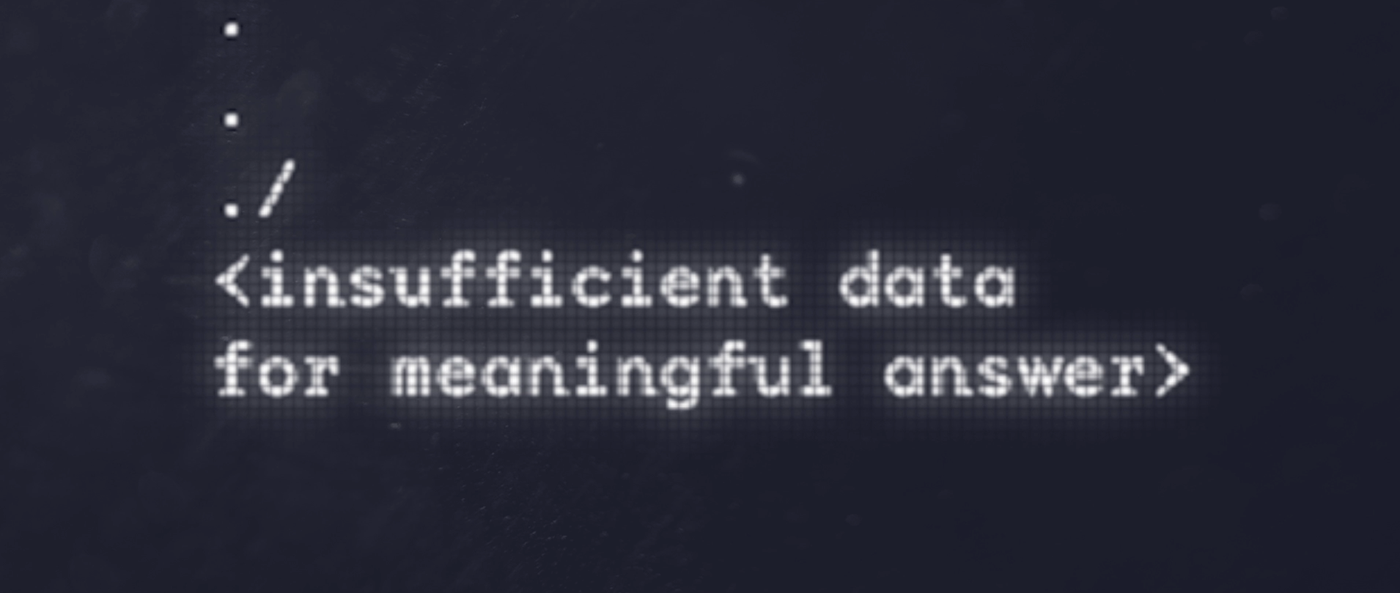
\includegraphics[width=0.6\textwidth]{./lq}				 
	\caption{Insufficient data.}		
	\label{img:ihuma}												 
\end{figure}													 
%----------------------------------------------------------

%--------- NEW SECTION ----------------------
\section{Assunto 1}
\label{sec:ass1}
\lipsum[1]



%---------------picture------------------------------------
% \begin{figure}
%     \centering
%     \subfigure[Figure A]{\label{fig:a}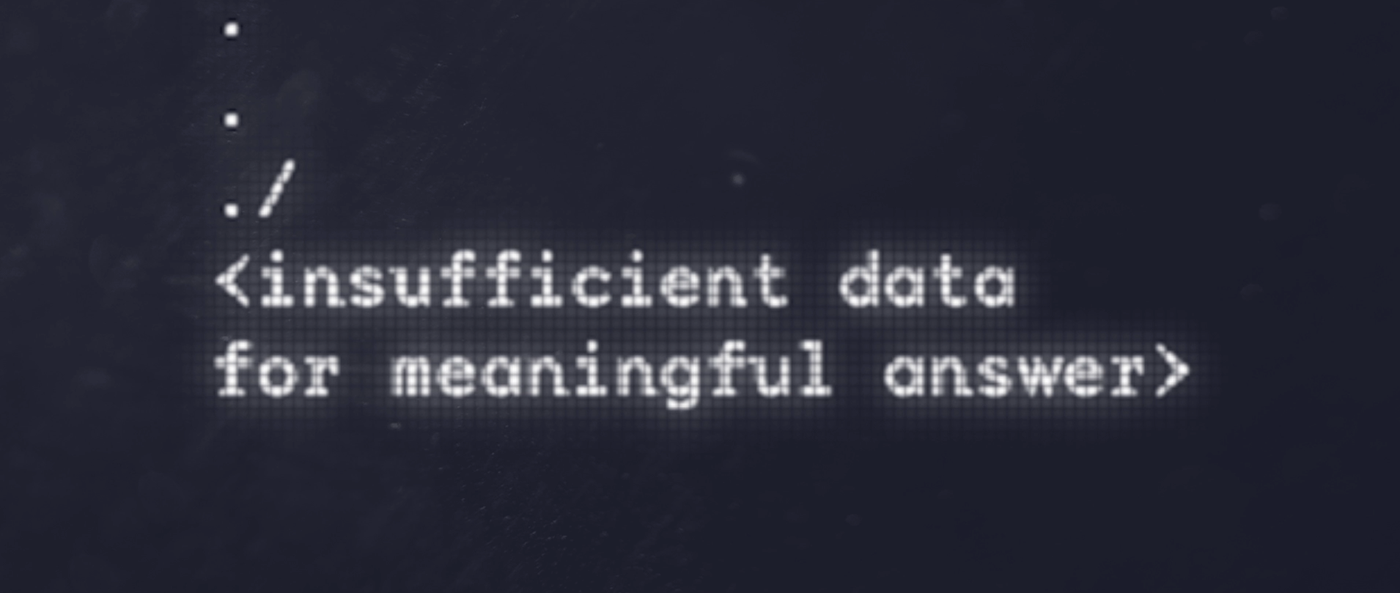
\includegraphics[width=60mm]{./lq}}
%     \subfigure[Figure B]{\label{fig:b}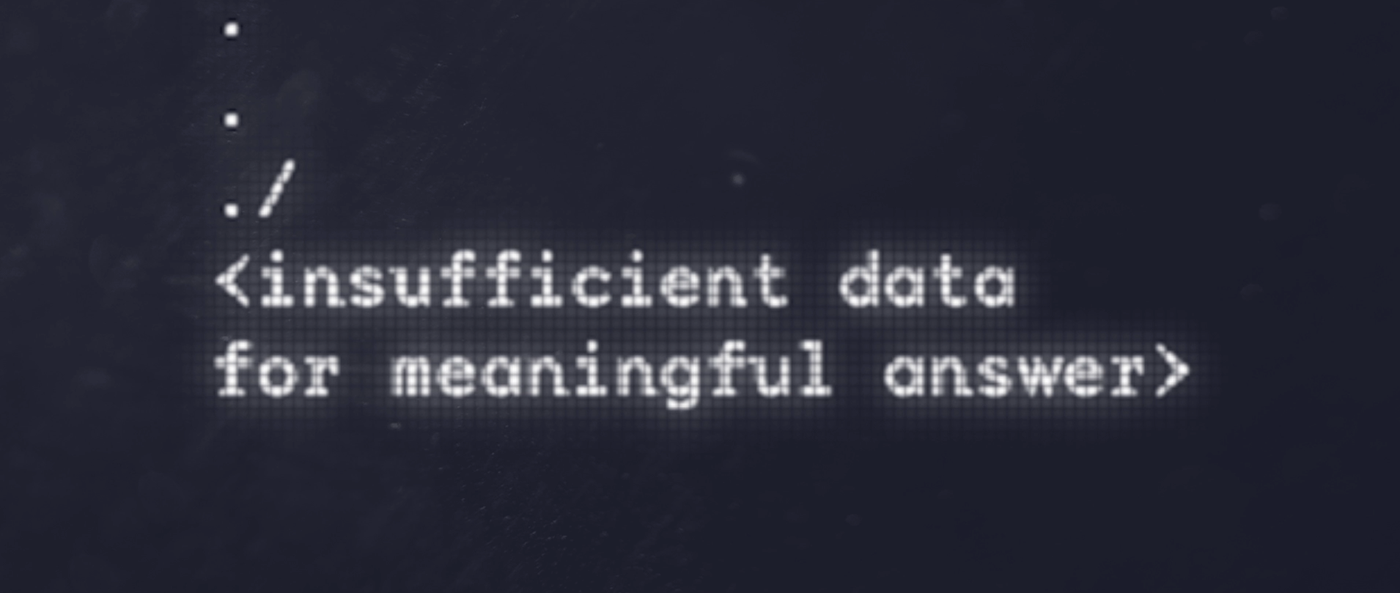
\includegraphics[width=60mm]{./lq}}
%     \subfigure[Figure C]{\label{fig:c}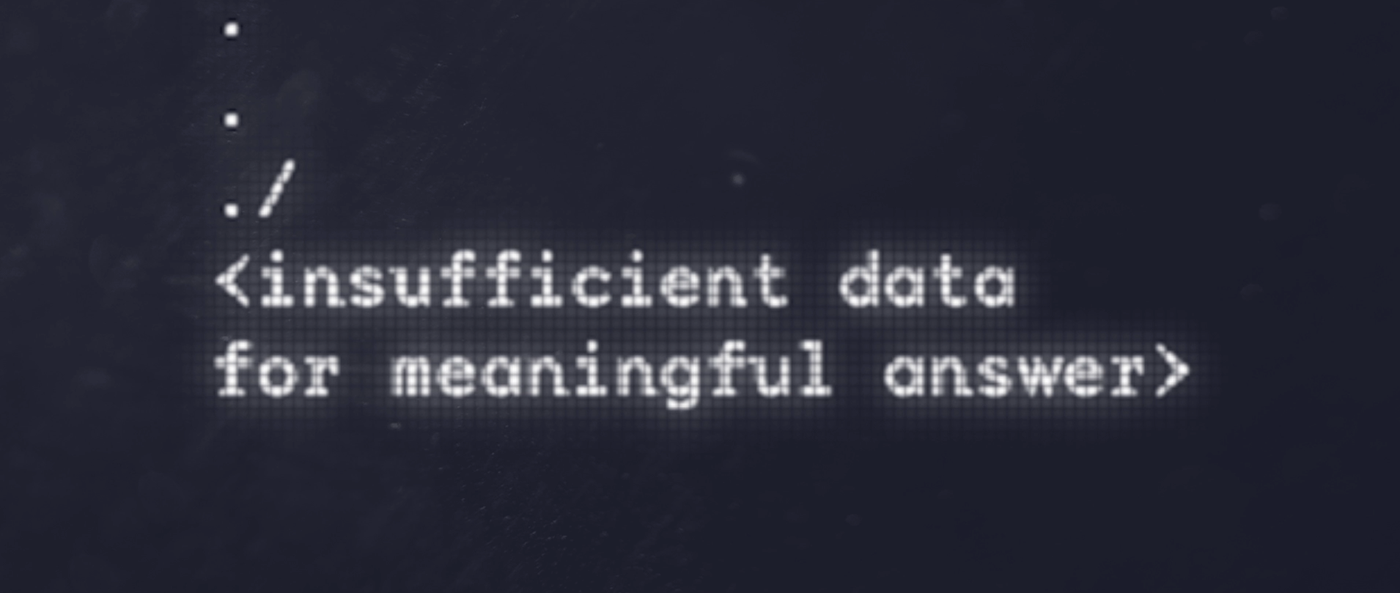
\includegraphics[width=\textwidth]{./lq}}
%     \caption{Three simple graphs}
%     \label{fig:three graphs}
% \end{figure}
%----------------------------------------------------------

\begin{figure}
    \centering
    \begin{subfigure}[b]{0.3\textwidth}
        \centering
        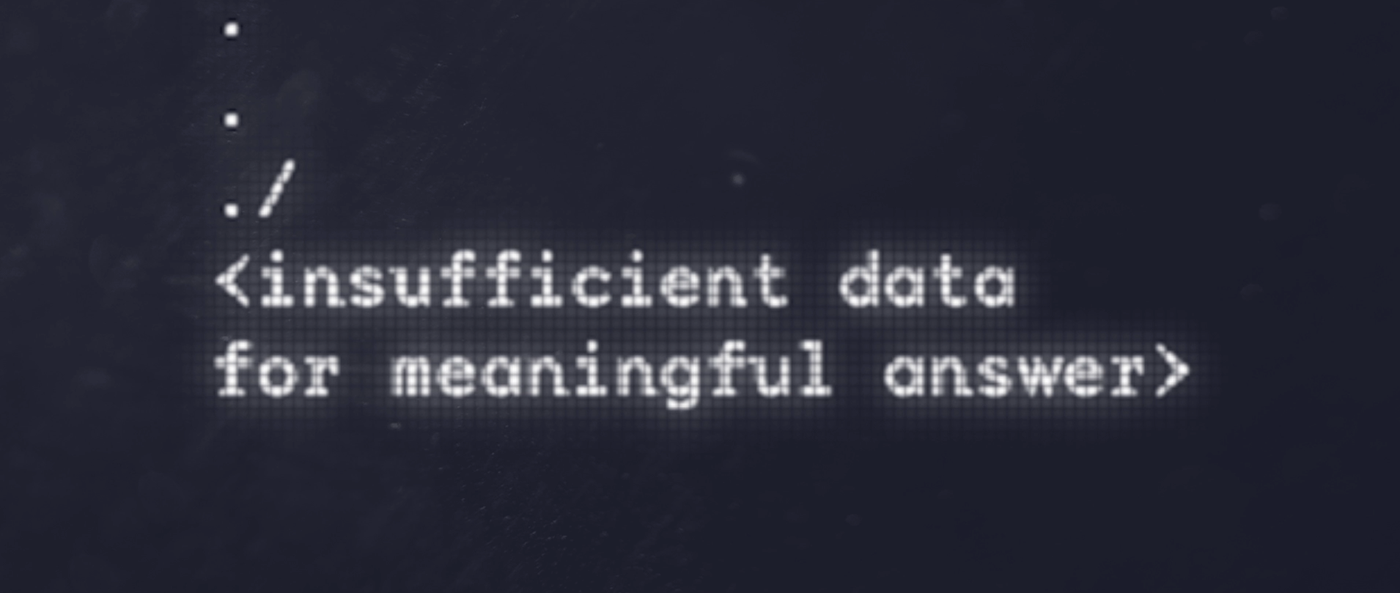
\includegraphics[width=\textwidth]{./lq}
        \caption{$y=x$}
        \label{fig:y equals x}
    \end{subfigure}
    \hfill
    \begin{subfigure}[b]{0.3\textwidth}
        \centering
        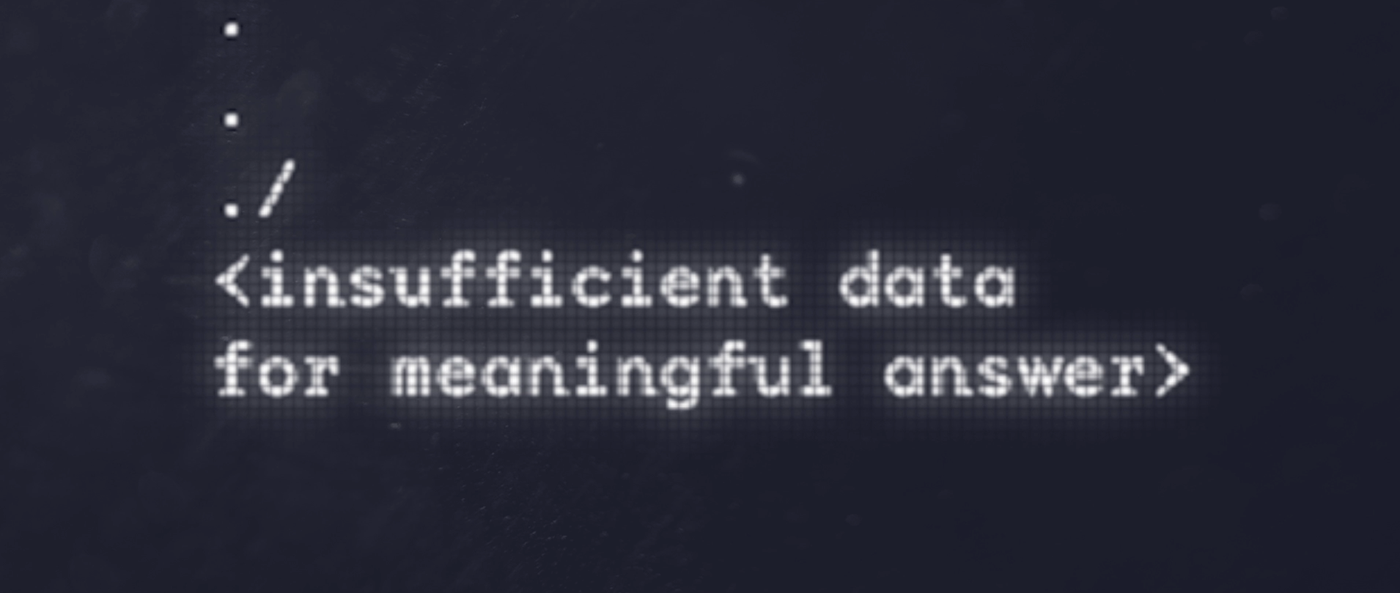
\includegraphics[width=\textwidth]{./lq}
        \caption{$y=3sinx$}
        \label{fig:three sin x}
    \end{subfigure}
    \hfill
    \begin{subfigure}[b]{0.3\textwidth}
        \centering
        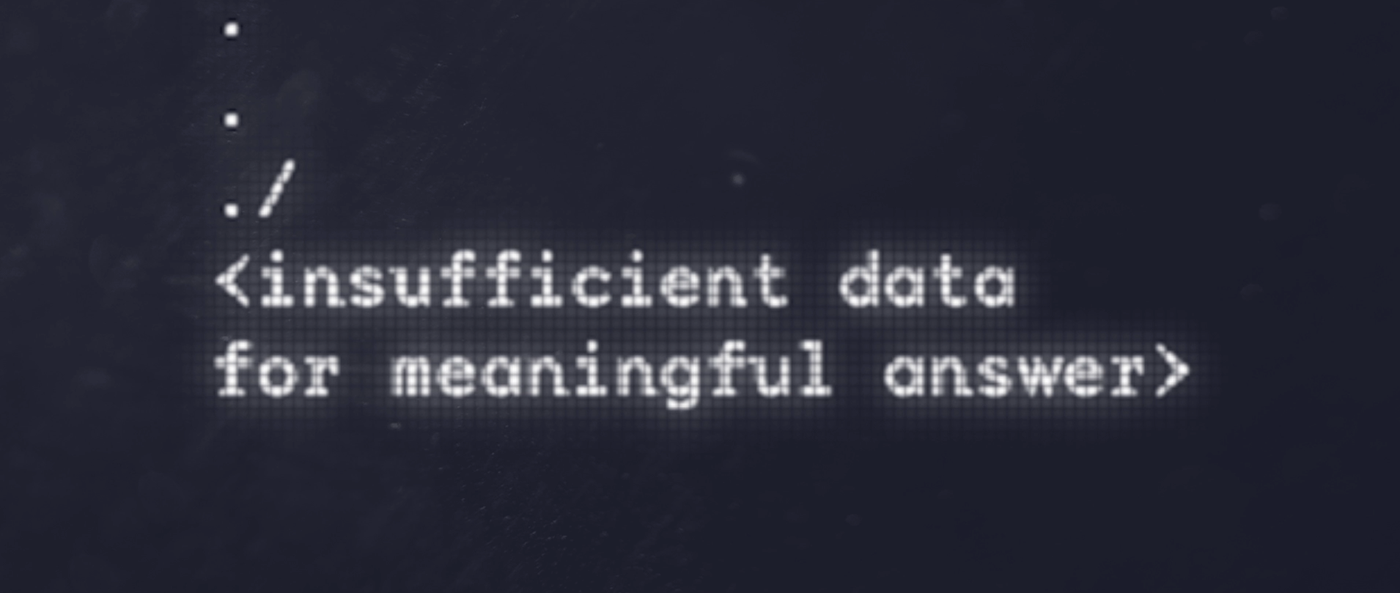
\includegraphics[width=\textwidth]{./lq}
        \caption{$y=5/x$}
        \label{fig:five over x}
    \end{subfigure}
       \caption{Three simple graphs}
       \label{fig:three graphs}
\end{figure}


%--------- NEW SECTION ----------------------
\section{Assunto 2}
\label{sec:ass2}
flkjasdlkfjasdlkfjs

\begin{table}[h]
    \begin{subtable}[h]{0.45\textwidth}
        \centering
        \begin{tabular}{l | l | l}
        Day & Max Temp & Min Temp \\
        \hline \hline
        Mon & 20 & 13\\
        Tue & 22 & 14\\
        Wed & 23 & 12\\
        Thurs & 25 & 13\\
        Fri & 18 & 7\\
        Sat & 15 & 13\\
        Sun & 20 & 13
       \end{tabular}
       \caption{First Week}
       \label{tab:week1}
    \end{subtable}
    \hfill
    \begin{subtable}[h]{0.45\textwidth}
        \centering
        \begin{tabular}{l | l | l}
        Day & Max Temp & Min Temp \\
        \hline \hline
        Mon & 17 & 11\\
        Tue & 16 & 10\\
        Wed & 14 & 8\\
        Thurs & 12 & 5\\
        Fri & 15 & 7\\
        Sat & 16 & 12\\
        Sun & 15 & 9
        \end{tabular}
        \caption{Second Week}
        \label{tab:week2}
     \end{subtable}
     \caption{Max and min temps recorded in the first two weeks of July}
     \label{tab:temps}
\end{table}
    \chapter{Materiais e Métodos}
\label{chap:mat}
Nas próximas seções estarão descritos os materiais e métodos aplicados para cada projeto realizado durante o curso de formação em Robótica e Sistemas Autônomos. 

\section{Desafio 1.0}
\label{sec:met_desafio1}
Este desafio foi feito individualmente, e ele foi realizado com o objetivo de programar o robô da \textit{Clearpath Robotics- Husky}, no ambiente de simulação do \textit{Gazebo}. A área de operação desse robô foi a área externa entre os prédios do CIMATEC 3 e 4. O \textit{Husky} tinha como missão explorar esse ambiente externo a procura de uma bola amarela, e ao identificar esta ele deveria ir até ela e parar de frente para mesma informando que a missão foi completada. Como nesse desafio foi realizada apenas a simulação, apenas o computador foi utilizado.  

%--------- NEW SECTION ----------------------
\section{Desafio 2.0}
\label{sec:met_desafio2}
O segundo desafio foi realizado em grupo composto por mim, Leonardo, Miguel e Vinícius, onde um manipulador deveria ser concebido desde sua fase inicial modelando toda sua estrutura e posteriormente realizada a simulação deste no \textit{Gazebo}, com a missão da câmera integrada ao manipulador identificar o \textit{ArUco} na caixa e pressionar o botão. Este desafio também foi realizada apenas a simulação, por isso apenas o computador foi utilizado.  

%--------- NEW SECTION ----------------------
\section{Desafio 2.2}
\label{sec:met_desafio2_2}
Este desafio foi para construir o modelo real do manipulador JeRoTimon modelado no desafio \ref{sec:met_desafio2}, realizado com a equipe composta por mim, Jean, Leonardo, Miguel, Vinícius e Rodrigo, onde o objetivo era o mesmo, reconhecer a \textit{tag ArUco} na caixa e pressionar o botão, só que dessa vez no ambiente real. Os materiais utilizados nesse desafio foram perfis de alumínio, motores \textit{Dynamixel}, câmera RGB modelo \textit{Teledyne Genie Nano C2590},  peças modeladas no \textit{OnShape} e impressas em \textit{ABS} por uma impressora 3D, conexões para alimentação e para comunicação

%--------- NEW SECTION ----------------------
\section{Desafio 2.5}
\label{sec:met_desafio2_5}
O desafio 2.5 foi realizado em equipe, a mesma do desafio \ref{sec:met_desafio2}, onde o robô programado foi o \textit{Darwin-OP} e este deveria realizar duas missões, a primeira, é a marcha, onde quatro robôs \textit{Darwin-OP} deveriam andar de forma sincronizada de um ponto a outro da pista de corrida. E a segunda missão foi realizada a programação para que os quatro robôs realizassem a corrida com revezamento, onde cada robô está posicionado numa parte específica da pista de corrida e ao chegar próximo um do outro eles mantém por um período a movimentação sincronizada depois o anterior para e o outro segue, igualmente a uma corrida com revezamento real.


%--------- NEW SECTION ----------------------
\section{Desafio 3.0}
\label{sec:met_desafio3}

%--------- NEW SECTION ----------------------
\section{Artigo do Ciclo 1}
\label{sec:met_artigo1}


%--------- NEW SECTION ----------------------
\section{Artigo do Ciclo 2}
\label{sec:met_artigo2}


    \chapter{Resultados}
\label{chap:result}
Nesta seção serão demonstrados os trabalhos realizados durante o período do curso de formação em Robótica e Sistemas Autônomos, identificando nos apêndices os relatórios, mapas mentais e apresentações realizadas. E nos textos são indicados os repositórios onde é possível verificar os códigos, os pré-requisitos para funcionar o pacote e o tutorial para realizar a simulação ou o modelo real.

%--------- NEW SECTION ----------------------
%\section{Programação do \textit{Turtlesim} no \textit{ROS} em \textit{Python}}
%\label{sec:testu}
%Como mencionado anteriormente, nas primeiras semanas foram inicializadas as atividades dentro da programação do curso onde neste primeiro momento começamos a etapa de absorção e desenvolvimento de conhecimentos que nos seriam requeridos durante todo o curso.
%No repositório \url{https://github.com/JessMotta/desafio_turtlesim_setpoint} encontra-se a primeira atividade desenvolvida, onde foi realizada a programação do \textit{Turtlesim}, no  \textit{ROS}, na linguagem de programação \textit{Python}. Este desafio teve por finalidade inicializar o contato com o \textit{ROS}, pois esse \textit{framework} é o mais utilizado na robótica, e a linguagem de programação \textit{Python} também é uma das mais utilizadas nessa área.
%O desafio constituia realizar a programação do \textit{Turtlesim} para que ele se movimentasse para locais específicos definidos pelo usuário.

%\section{Aprendizado do \textit{OpenCV}}
%\label{sec:intsis}
%O \textit{OpenCV (Open Source Computer Vision)} é uma biblioteca de código aberto que tem por finalidade tornar mais acessível para desenvolvedores a visão computacional. Nesse repositório \url{https://github.com/JessMotta/opencv_learning} é possível encontrar o código estruturado em \textit{Python} e os conhecimentos obtidos no primeiro contato com \textit{OpenCV} e suas possibilidades de aplicação. Além do que nos foi orientado que essa biblioteca seria muito utilizada para os projetos que iríamos desenvolver na área de robótica e sistemas autônomos. 

%--------- NEW SECTION ----------------------
%\section{Desafio 1.0 }
%\label{sec:desafio_1}
%O primeiro desafio, disponível no repositório \url{https://github.com/JessMotta/challenge_ws}, nele é possível verificar os pré-requisitos e o que é necessário para executar a simulação. Na Figura \ref{fig:cimatec3_4} tem-se o ambiente externo entre os prédios CIMATEC 3 e 4.   


%\begin{figure}[H]
 %   \caption{Área externa do CIMATEC 3 e 4, ambiente de simulação do \textit{Gazebo}}
  %  \centering
   % 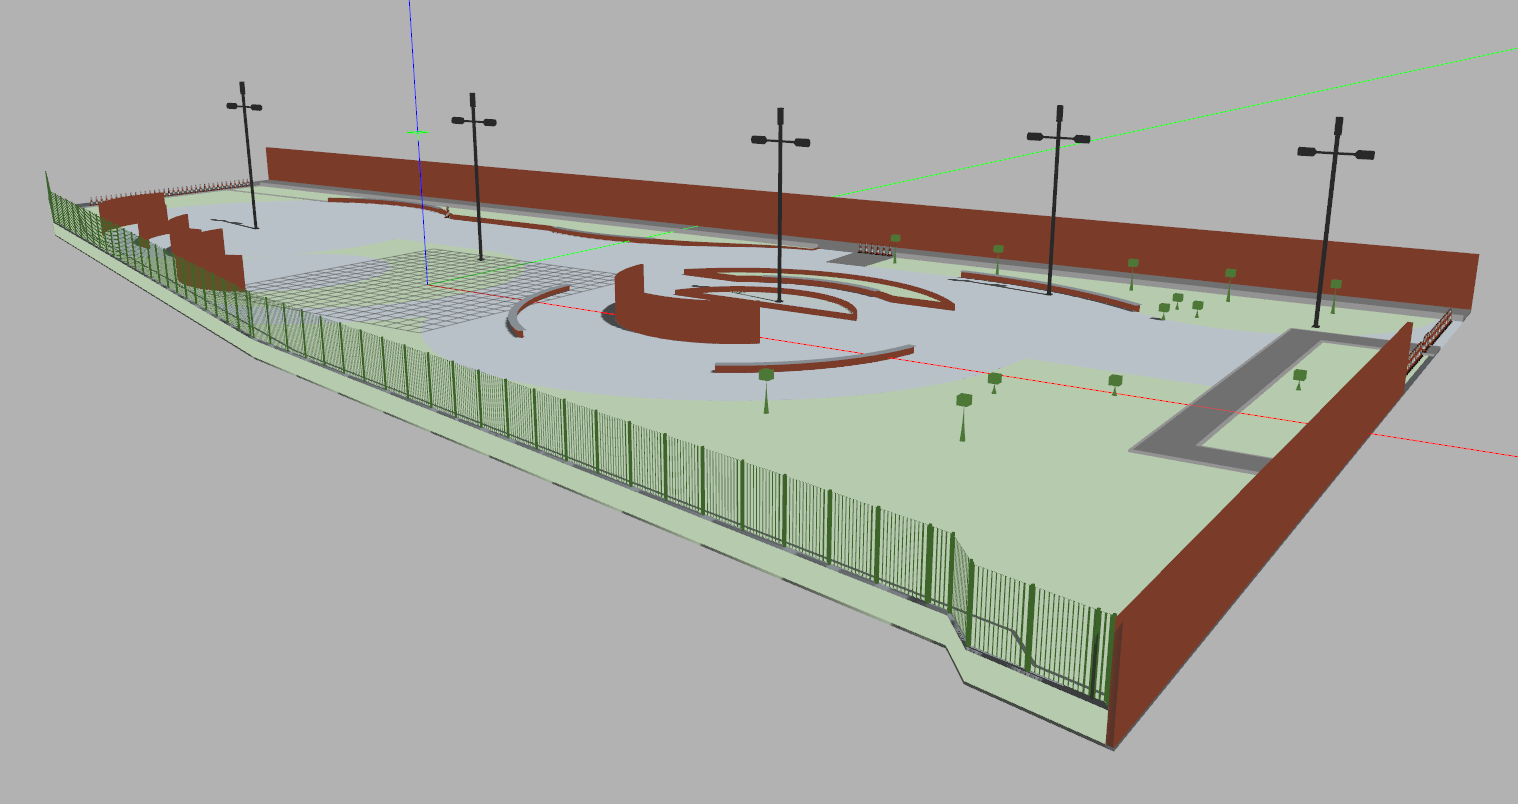
\includegraphics[width= \textwidth]{Figures/cimatec4.png}
    %\caption*{Fonte: Grupo de Formação em Robótica e Sistemas Autônomos}
    %\label{fig:cimatec3_4}
%\end{figure}



\section{Desafio 2.0 }
\label{sec:desafio_2}
Este desafio está disponível no repositório \url{https://github.com/Brazilian-Institute-of-Robotics/timon\_hm\_manipulator}, onde neste também tem os pré-requisitos e o tutorial de como executar a simulação. Na Figura \ref{fig:manipulador_simulacao} é possível verificar o manipulador JeRoTimon no ambiente de simulação do \textit{Gazebo}. No apêndice encontra-se o relatório elaborado para esse desafio, com todas as especificações do mesmo, o estado da arte e as informações dos motores utilizados.

\begin{figure}[H]
    \caption{Realização do desafio no ambiente de simulação do \textit{Gazebo}}
    \centering
    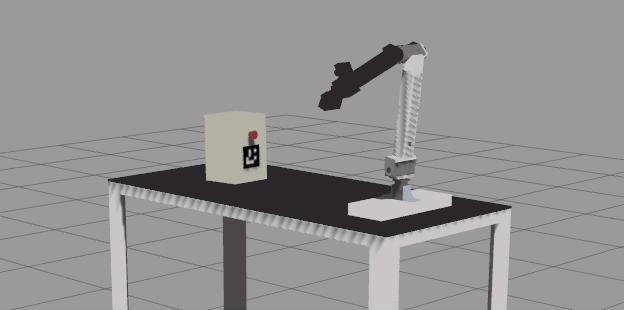
\includegraphics[width= \textwidth]{Figures/manipulador_simulacao.png}
    \caption*{Fonte: Grupo de Formação em Robótica e Sistemas Autônomos}
    \label{fig:manipulador_simulacao}
\end{figure}



\section{Desafio 2.2 }
\label{sec:desafio_2_2}
Este desafio está no mesmo repositório \url{https://github.com/Brazilian-Institute-of-Robotics/timon\_hm\_manipulator} onde tem a simulação, há também uma parte reservada para o a utilização em ambiente real. Na Figura \ref{fig:manipulador_real} é demonstrado o manipulador JeRoTimon real e a caixa, e o mesmo executando a missão de pressionar o botão. O relatório elaborado para esse desafio, é o mesmo do \ref{sec:desafio_2}, onde é possível encontrar maiores detalhes do projeto real.



\begin{figure}[H]
    \caption{Realização do desafio no ambiente real}
    \centering
    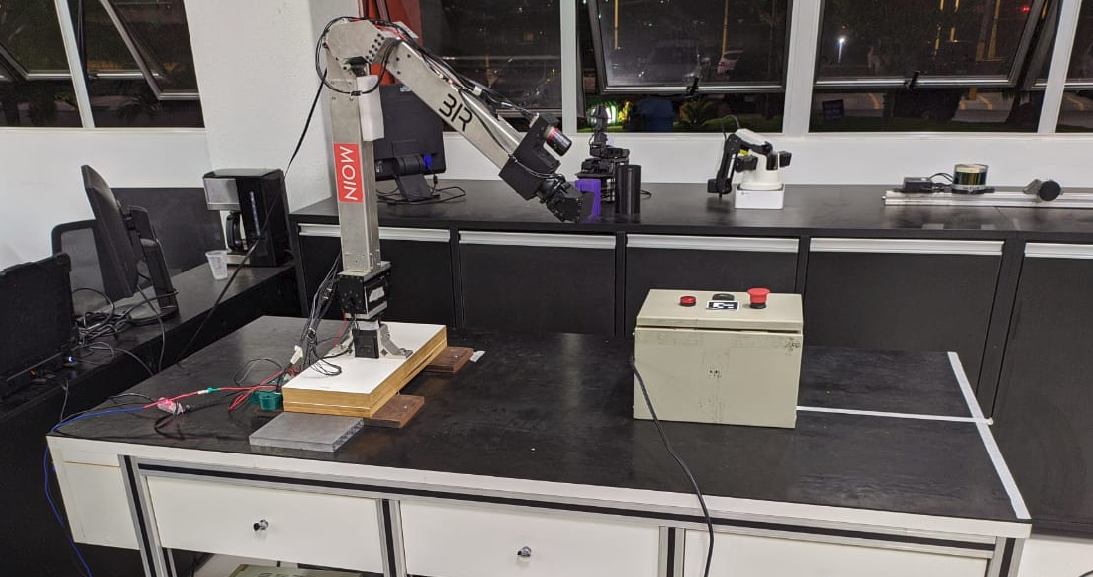
\includegraphics[width= \textwidth]{Figures/manipulador_real.png}
    \caption*{Fonte: Grupo de Formação em Robótica e Sistemas Autônomos}
    \label{fig:manipulador_real}
\end{figure}



\section{Desafio 2.5}
\label{sec:desafio_2_5}
O desafio 2.5, disponível no repositório \url{https://github.com/Brazilian-Institute-of-Robotics/timon_hm-2-5} foi realizado em equipe, a mesma do desafio \ref{sec:desafio_2}, onde o robô programado foi o \textit{Darwin-OP} e este deveria realizar duas missões, a primeira, é a marcha  


\section{Desafio 3.0}
\label{sec:desafio_3_0}

\section{Analíse estatística R\&R da simulação do robô Darwin OP }
\label{sec:analise_darwin}

testes

\section{Planejamento de Experimentos (DOE) -Helicóptero de Papel (TIMON-HM)}
\label{sec:analise_doe}
    \chapter{Conclusão}
\label{chap:conc}

De forma geral, o programa de formação proporcionou o desenvolvimento de conhecimentos e habilidades requeridas nas áreas de robótica e sistemas autônomos. Os resultados derivados dos projetos, foram expostas no cápitulo \ref{chap:result} onde envolveu um enorme aprendizado de planejamento, execução e entrega de projetos.
Este documento mostrou o desenvolvimento de um especialista no curso de formação em Robótica e Sistemas Autônomos, que foi formado com base nas ferramentas utilizadas para modelagem, simulação e construção real desses sistemas, e que são usadas no mundo todo nessa área de Robótica e Sistemas Autônomos, nas linguagens de programações fundamentais como \textit{C++, Python} e \textit{R}, sobre como os estudos estatísticos são aplicados para fazer análise dos projetos, e saber elaborar o planejamento, direcionar a execução e entregar os resultados aos clientes do projetos propostos. 


    % include more chapters ...
%
% ----------------------------------------------------------------------------
% Include thesis appendices
    \begin{thesisappendices}
        \includepdf[pages={1-134}]{Appendices/report_manipulador_jerotimon.pdf}
        % Thesis Appendix -------------------------------------------------------

\chapter{Diagramas mecânicos}
\label{Append:diagmec}



        % Thesis Appendix -------------------------------------------------------

\chapter{Diagramas eletro-eletrônicos}
\label{Append:diagele}



        % Thesis Appendix -------------------------------------------------------

\chapter{Logbook}
\label{Append:log}



    \end{thesisappendices}
%
% ----------------------------------------------------------------------------
% Configurar as referencias bibliograficas
	\renewcommand\bibname{Referências}
    \addcontentsline{toc}{chapter}{Referências}
    \bibliography{References/referencias}
%
% ----------------------------------------------------------------------------
% Finishing him
    \include{Others/ultimafolha}
\end{document}
%
% -------------------------------------------------------------------------------
% Aqui termina a formatação para o documento.
% In God We Trust. All Other Bring Data. 
%
% -------------------------------------------------------------------------------